%! TEX root = main.tex

\subsection{Mass source: rupture points}

We model a rupture point with a point inflow source feeding fluid into the domain.
Oil leak rates are specified in $m^3/s$, while the mass source term ($I$) requires $m^2/s$.
We calculate the source term by dividing the actual flow rates with the grid cell area at each AMR level.
Though this approach is simple and robust in practice, theoretically speaking, its numerical stability is still unclear when combined with the AMR algorithms in \geoclaw.

The leak rates can be modeled with a three-stage constant profile.
First, at the beginning of an incident, the high pressure from the upstream causes a high flow rate.
The leak rate is almost a constant due to the upstream constant pressure.
Second, once the pipeline operator identifies the pipeline section containing the breaking location, the operator shuts down the valves controlling that section.
The remaining oil in that section keeps flowing out.
The rate at this stage, theoretically, decreases along with time because the pressure continues to decrease.
In this work, however, we still model this stage with a constant for model simplicity.
As the real rate profile at this stage depends on many factors (such as the types of breakage, fluid properties, or operation conditions), there may not be a single model that can apply to all types of rupture events.
Finally, after the oil in the affected section is completely drained out, or once the pressure in the pipeline is not high enough, the leak rate of the point source becomes zero.

Given a specific location of breakage, the time span and the flow rate of each stage may be estimated with model predictions (\cite{abhulimen_liquid_2004}) or, in common practice, rely on the inputs from field experts.
Figure \ref{fig:outflow-profile} shows an example profile 

\begin{figure}
    \centering
    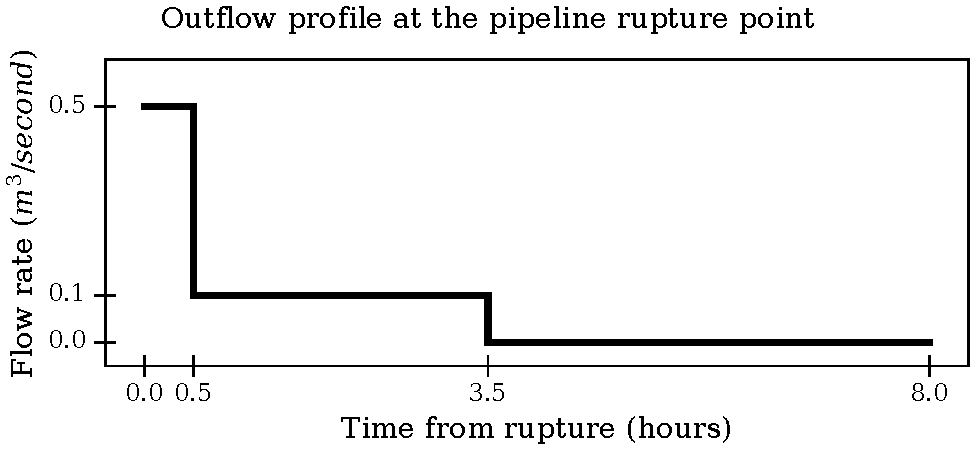
\includegraphics[width=0.9\linewidth]{landspill-outflow-profile}
    \caption{Outflow profile at the pipeline rupture point}\label{fig:outflow-profile}
\end{figure}
